\subsection{Particle Position Reconstruction}
Each detector is not capable of measuring the position of a detected particle along the axes parallel to its width (15.24~cm) or depth (3.81~cm), which contributes $\pm3^{\circ}$ to the total angular uncertainty.
The position of a detected particle along the 76.2~cm length of the scintillator is calculated using the timing difference of signals from both of a detector's PMTs.
Assuming that scintillation light travels from an initial point, let it be $x$~cm from the center of a scintillator, to both PMTs at a velocity that is constant with respect to the scintillator's length-wise axis, then the difference between the times at which the light will reach each PMT ($\Delta t^{PMTs}$) is given by:
\begin{equation}
\label{eq:PMTDiff1}
\begin{split}
\Delta t^{PMTs} & = t^{PMT_1}-t^{PMT_2} \\ 
& = \frac{(L/2 + x) n_{\text{eff}}}{c} - \frac{(L/2-x) n_{\text{eff}}}{c} \\
& = 2x \frac{n_{\text{eff}}}{c}  \, .
\end{split}
\end{equation}
Solving for $x$ gives 
\begin{equation}
\label{eq:position}
x = \frac{c}{2n_{\text{eff}}} \Delta t^{PMTs} \, ,
\end{equation}
where $t^{PMT_{1}}$ and $t^{PMT_{2}}$ are the times of signals from each of a detector's PMTs relative to the accelerator gun pulse, $L$ is the length of the scintillator, $c$ is the speed of light, $n_{\text{eff}}$ is the effective index of refraction of the scintillation material.
A linear least squares  fit between $x$ and $\Delta t^{PMTs}$ was performed on data gathered using coincident photons emitted by a collimated $^{60}$Co source, as described in the previous section.
The resulting fit parameters, seen in Fig.~\ref{fig:PMTDifference}, are used to find the position of detected particles.
\begin{figure}[]
    \centering    
    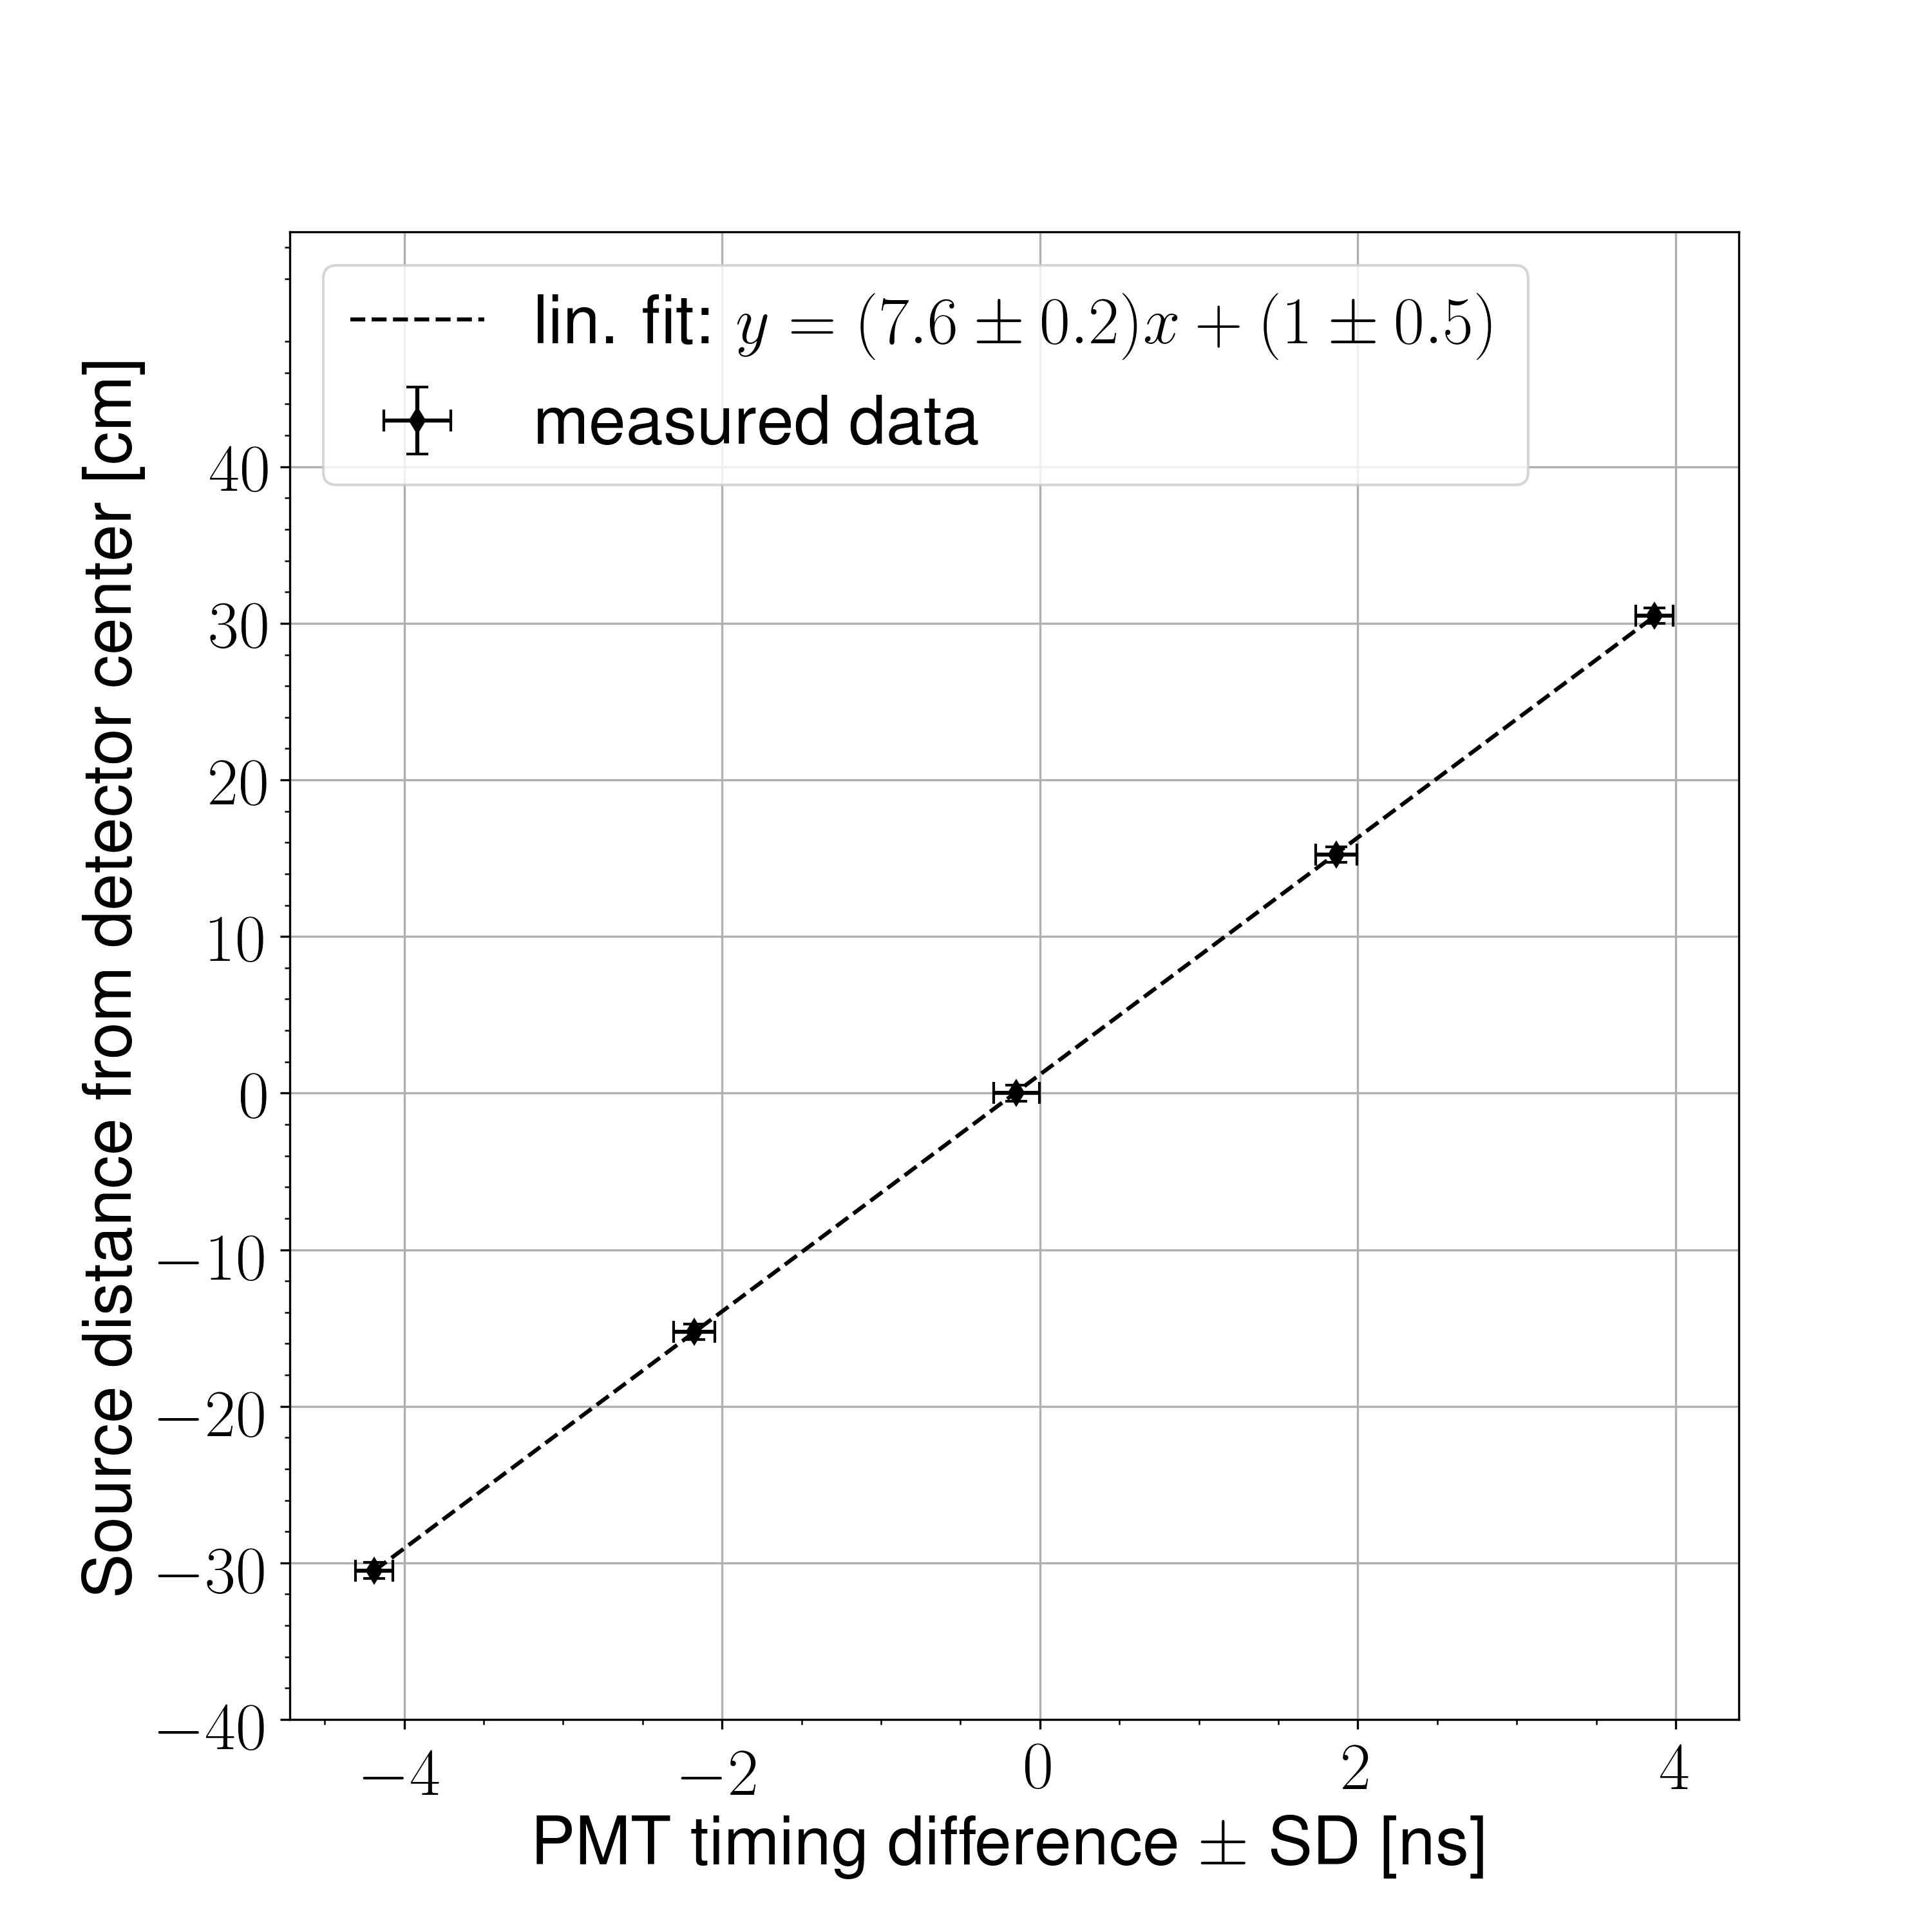
\includegraphics[width = \figsize\textwidth]{PMTDifference.png}
    \caption{
    A collimated $^{60}$Co source is used to produce photon events at five different positions along the scintillator.
    The mean PMT timing difference of events at each position varies linearly with respect to the distance of the $^{60}$Co source from the center of the detector. 
    The result of a linear least squares fit to this data is used to calculate the position of detected particles along the length of each scintillator.
    }
    \label{fig:PMTDifference}
\end{figure}

Using the slope of the linear fit in Fig.~\ref{fig:PMTDifference}, along with Eq.~\ref{eq:position}, an effective index of refraction of the scintillation material is calculated to be 2.0.
This index of refraction is said to be ``effective" because its measurement is sensitive only to the scintillation light's average speed projected onto the axis parallel to the scintillator's longest dimension, which is equal to the intrinsic speed of light in the material only when said light is traveling parallel to the scintillator's length.
While the detection of scintillation light by both PMTs favors light paths which are parallel or nearly-parallel to the scintillator's length, there is some reflection of detected scintillation light from the boundaries of the scintillator.
This effect contributes to the $\pm9$~cm measurement uncertainty in particle position reconstruction.
As a result of these effects, the index of refraction measured here is $\sim{25}\%$ greater than the true value for the scintillation material.  
